% !TeX root = ..\main.tex
%%%%%%%%%%%%%%%%%%%%%%%%%  
\section{Hạn chế của đề tài}
\hspace{0.5cm} Khi thực hiện chuyển đổi BPMN thành BPEL, các User Task trong BPMN sẽ được chuyển thành Human Task trong BPEL, tuy nhiên việc thực hiện các Human Task này yêu cầu phải thông qua ứng dụng BPM Worklist và được thực hiện bởi tài khoản được cung cấp từ Weblogic Server của Oracle và không thể được thực hiện từ xa (thông qua Http API), do đó việc thực hiện các Human Task chỉ phù hợp với các hệ thống quản lý nội bộ và làm việc trực tiếp với ứng dụng từ Oracle. \\

Vì vậy, trong đề tài này, nhóm chỉ thực hiện xây dừng các quy trình BPEL mà trong đó hệ thống thực hiện tự động hoàn toàn mà không có các hành động xen giữa quy trình của con người để phù hợp với hệ thống bán hàng.


%%%%%%%%%%%%%%%%%%%%%%%%%
\section{Những nhiệm vụ đã hoàn thành cho đề tài}
Trong giai đoạn đồ án chuyên ngành, nhóm đã hiện thực được những công việc như sau:
\begin{itemize}
    \item Tìm hiểu về quy trình nghiệp vụ và các công cụ sử dụng để mô hình hóa quy trình nghiệp vụ.
    \item Tìm hiểu về các chuyển đổi từ lược đồ BPMN sang BPEL để áp dụng cho tự động hóa quy trình nghiệp vụ.
    \item Phân tích yêu cầu chức năng và phi chức năng của hệ thống.
    \item Xây dựng và mô hình hóa được quy trình nghiệp vụ cho hệ thống.
    \item Hoàn thành thiết kế kiến trúc cho hệ thống: lược đồ use-case, cơ sở dữ liệu, lược đồ class, giao diện người dùng.
    \item  Lựa chọn công nghệ để hiện thực front-end và back-end cho hệ thống.
\end{itemize}
 
 
\section{Kế hoạch cho giai đoạn đồ án tốt nghiệp}
 
\begin{figure}[h]
    \begin{center}
        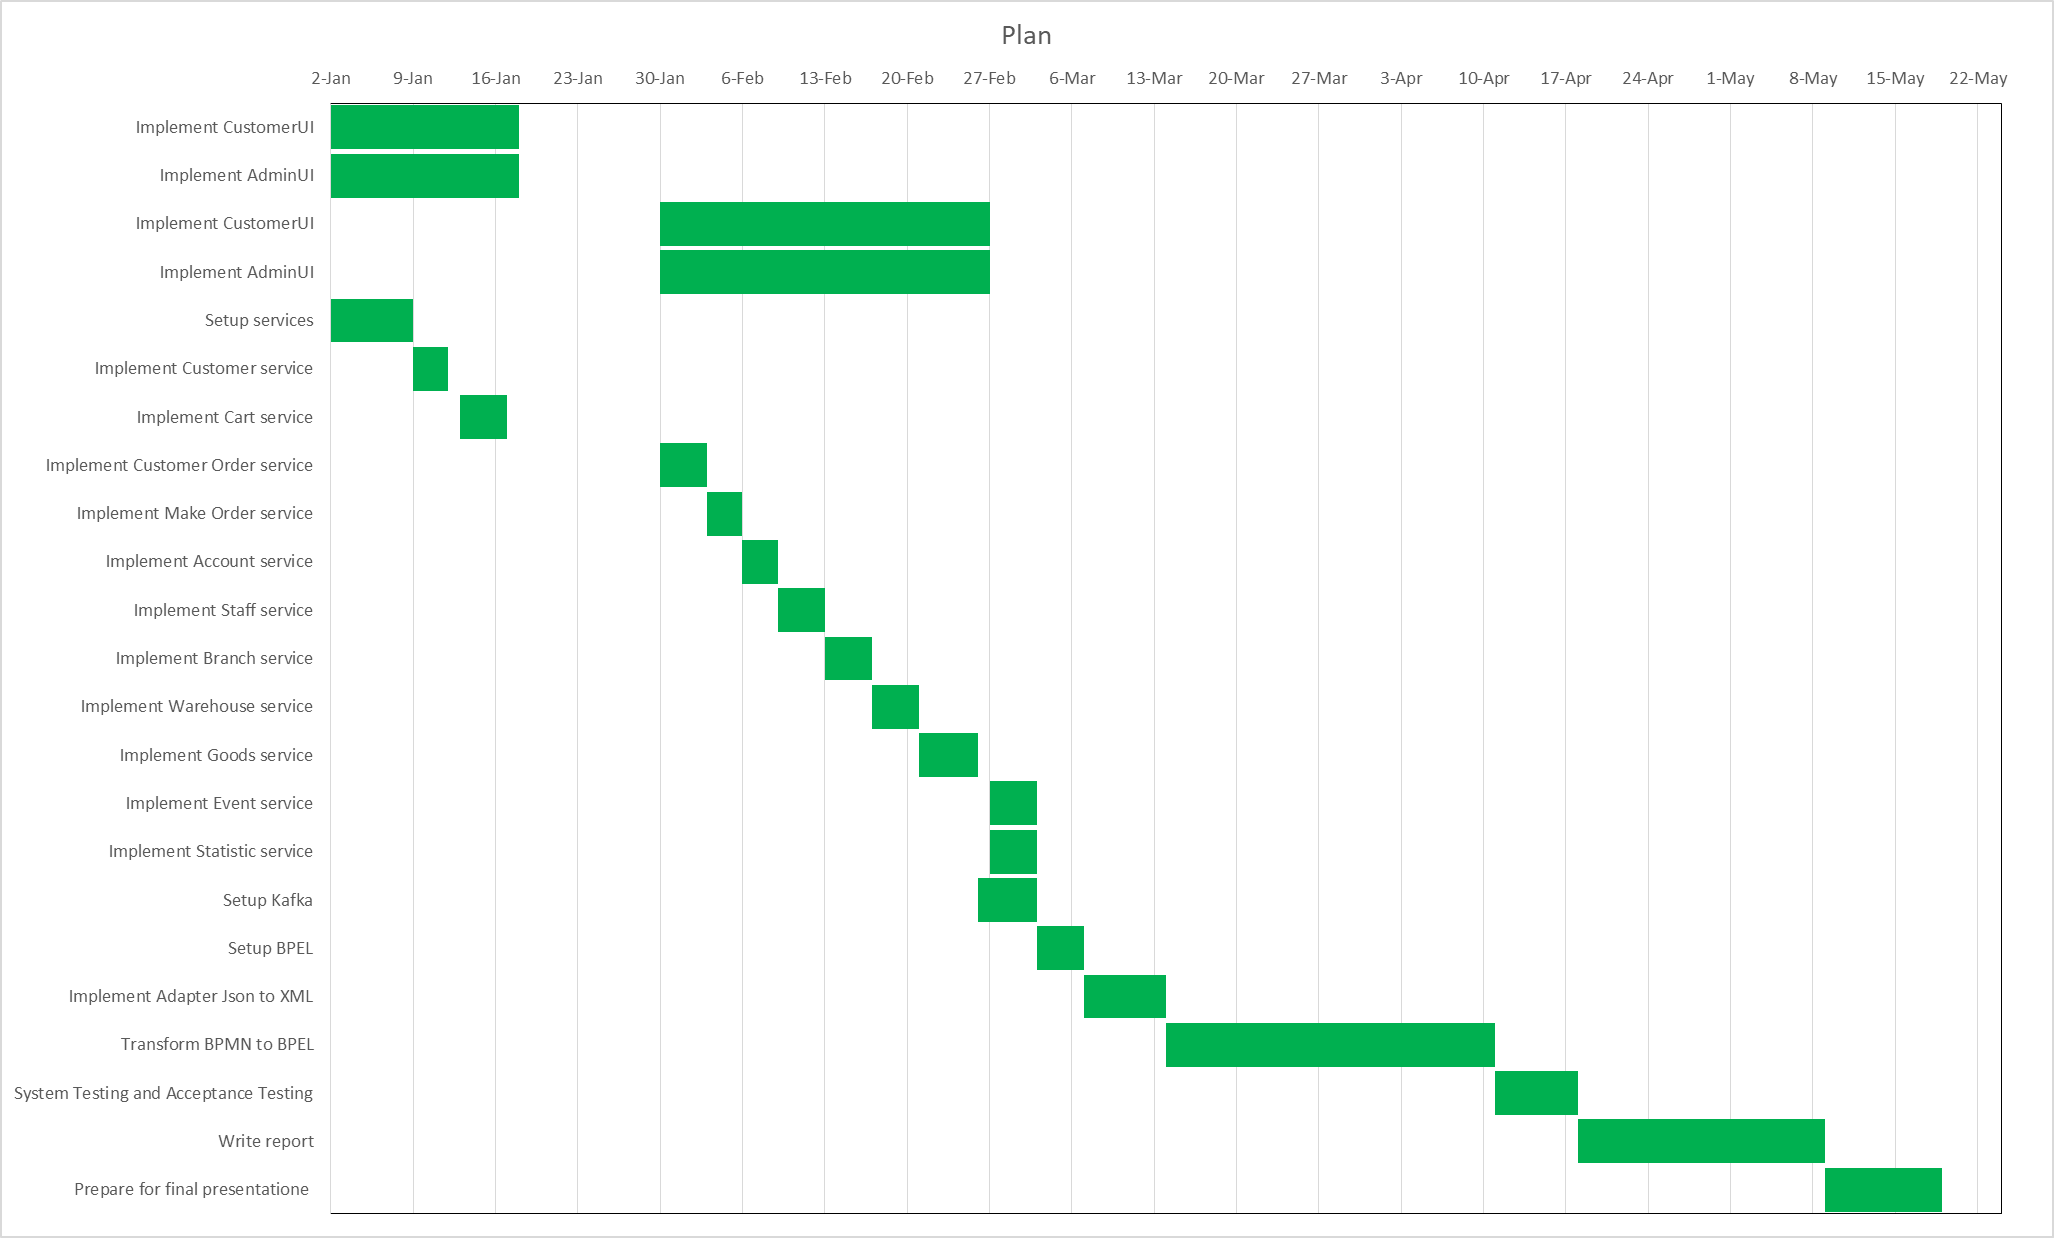
\includegraphics[width=14cm]{img/plan.png}
    \end{center}
    \caption{Biểu đồ Gantt cho kế hoạch đồ án tốt nghiệp}
\end{figure}
 
Lưu ý: Khoảng trống từ ngày 16/1 đến 29/1 là thời gian nghỉ tết

\newpage
\section{Bảng phân công công việc trong giai đoạn đồ án tốt nghiệp}
{
\setlength\extrarowheight{6pt}
\begin{longtable}{| p{2cm} | p{2cm} | p{10cm} |}

	\hline
	\textbf{Bắt đầu} & \textbf{Hạn} & \textbf{Công việc} \\
	\hline
	02/01/2023 & 08/01/2022 & 
    - Phong: Setup môi trường cho CustomerUI và hiện thực layout. 
    \newline
    - Hiển: Setup môi trường cho AdminUI và hiện thực layout.
    \newline
    - Thọ: Setup môi trường cho backend, khởi tạo các service và đảm bảo giao tiếp giữa các service. \\
	\hline
	09/01/2023 & 16/09/2022 & 
    - Phong: Hiện thực Login page - Register page và Reset Password page. 
    \newline
    - Hiển: Hiện thực Branch page - Branch detail page - Order page - Order detail page. 
    \newline
    - Thọ: Hiện thực Customer service và Cart service. \\
	\hline
	30/01/2023 & 05/02/2022 & 
    - Phong: Hiện thực Home page - List Product page. 
    \newline
    - Hiển: Hiện thực Event page - Event detail page - Goods page - Goods detail page, Goods Edit page. 
    \newline
    - Thọ: Hiện thực Customer Order service. \\
	\hline
	06/02/2023 & 12/02/2022 & 
    - Phong: Hiện thực Product Detail page - Cart page. 
    \newline
    - Hiển: Hiện thực Staff page - Staff Detail page - Staff Request page. 
    \newline
    - Thọ: Hiện thực Account service và Staff service. \\
	\hline
	13/02/2023 & 19/02/2022 & 
    - Phong: Hiện thực Payment page - Manager Order page. 
    \newline
    - Hiển: Hiện thực Account page, Account Detail page. 
    \newline
    - Thọ: Hiện thực Branch service và Warehouse service. \\
	\hline
	20/02/2023 & 26/02/2022 & 
    - Phong: Hiện thực Order Detail page và Customer Info page. 
    \newline
    - Hiển: Hiện thực Warehouse page - Statistic page. 
    \newline
    - Thọ: Hiện thực Goods service. \\
	\hline
	27/02/2023 & 05/03/2022 & 
    - Phong: Refactor code cho CustomerUI, hiện thực Event service. 
    \newline
    - Hiển: Refactor code cho AdminUI, hiện thực Statistic service. 
    \newline
    - Thọ: Setup kafka. \\
	\hline
	06/03/2023 & 12/03/2022 & 
    - Tất cả thành viên: Setup BPEL, hiện thực adapter chuyển đổi từ JSON sang XML. \\
	\hline
	13/03/2023 & 19/03/2022 & 
    - Tất cả thành viên: Hiện thực chuyển đổi từ BPMN sang BPEL. \\
	\hline
	20/03/2023 & 26/03/2022 & 
    - Tất cả thành viên: Tiếp tục hiện thực chuyển đổi từ BPMN sang BPEL. \\
	\hline
	27/03/2023 & 02/04/2022 & 
    - Tất cả thành viên: Tiếp tục hiện thực chuyển đổi từ BPMN sang BPEL. \\
	\hline
	03/04/2023 & 09/04/2022 & 
    - Tất cả thành viên: Tiếp tục hiện thực chuyển đổi từ BPMN sang BPEL. \\
	\hline
	10/04/2023 & 16/04/2022 & 
    - Tất cả thành viên: Tổng hợp hệ thống. \\
	\hline
	17/04/2023 & 23/04/2022 & 
    - Tất cả thành viên: Thực hiện system testing và acceptance testing. \\
	\hline
	24/04/2023 & 30/04/2022 & 
    - Tất cả thành viên: Viết báo cáo.
    \newline
    - Phong: Chỉnh sửa CustomerUI, Event service, Cart service, Customer service khi nhận được feedback và cần cải thiện. 
    \newline
    - Hiển: Chỉnh sửa AdminUI, Staff service, Account service, Branch service, Statistic service khi nhận được feedback và cần cải thiện. 
    \newline
    - Thọ: Chỉnh sửa Kafka, Warehouse service, Order service, Goods service khi nhận được feedback và cần cải thiện. \\
	\hline
	01/05/2023 & 07/05/2022 & 
    - Tất cả thành viên: Chỉnh sửa báo cáo và chuẩn bị slide thuyết trình.
    \newline
    - Phong: Chỉnh sửa CustomerUI, Event service, Cart service, Customer service khi nhận được feedback và cần cải thiện. 
    \newline
    - Hiển: Chỉnh sửa AdminUI, Staff service, Account service, Branch service, Statistic service khi nhận được feedback và cần cải thiện. 
    \newline
    - Thọ: Chỉnh sửa Kafka, Warehouse service, Order service, Goods service khi nhận được feedback và cần cải thiện. \\
	\hline
	08/05/2023 & 14/05/2022 & 
    - Tất cả thành viên: Chỉnh sửa, cập nhật báo cáo và slide thuyết trình.
    \newline
    - Phong: Chỉnh sửa CustomerUI, Event service, Cart service, Customer service khi nhận được feedback và cần cải thiện. 
    \newline
    - Hiển: Chỉnh sửa AdminUI, Staff service, Account service, Branch service, Statistic service khi nhận được feedback và cần cải thiện. 
    \newline
    - Thọ: Chỉnh sửa Kafka, Warehouse service, Order service, Goods service khi nhận được feedback và cần cải thiện. \\
	\hline
	15/05/2023 & 21/05/2022 & 
    - Tất cả thành viên: Chỉnh sửa, cập nhật báo cáo và slide thuyết trình.
    \newline
    - Phong: Chỉnh sửa CustomerUI, Event service, Cart service, Customer service khi nhận được feedback và cần cải thiện. 
    \newline
    - Hiển: Chỉnh sửa AdminUI, Staff service, Account service, Branch service, Statistic service khi nhận được feedback và cần cải thiện. 
    \newline
    - Thọ: Chỉnh sửa Kafka, Warehouse service, Order service, Goods service khi nhận được feedback và cần cải thiện. \\
	\hline
	22/05/2023 & 29/05/2022 & 
    - Tất cả thành viên: Chỉnh sửa slide và thực hiện phản biện cho đề tài. \\
	\hline
	29/05/2023 & 02/06/2022 & 
    - Tất cả thành viên: Chỉnh sửa slide và bảo vệ đồ án tốt nghiệp. \\
	\hline

\end{longtable}
}

%%%%%%%%%%%%%%%%%%%%%%%%%
% \subsection{Phân chia công việc}
